\newpage
\section{量子比特路由与映射联合优化}
\label{sec:routing-mapping}

\subsection{问题定义}

量子比特路由（Quantum Circuit Routing）是将逻辑量子电路映射到物理量子硬件的过程。由于 NISQ 设备中只有相邻的物理量子比特可以执行双量子比特门（如 CNOT），当逻辑门操作的两个量子比特在物理上不相邻时，必须插入 SWAP 门来交换量子比特的位置。每次 SWAP 操作引入额外噪声并增加电路深度，因此目标是在满足物理约束的前提下，最小化 SWAP 数量或最大化最终保真度。

更形式化地，给定：
\begin{itemize}
  \item 逻辑电路 $C$ 包含 $n$ 个逻辑量子比特和一系列门操作
  \item 物理拓扑 $G = (V, E)$ 包含 $m \geq n$ 个物理量子比特，$E$ 为相邻边集
  \item 初始映射 $\pi: [n] \to [m]$ 将逻辑量子比特映射到物理位置
\end{itemize}

每一步，智能体从 $E$ 中选择一条边 $(p,q)$ 执行 SWAP 操作，这一操作交换物理量子比特 $p$ 和 $q$ 上的内容。在 SWAP 后，所有前置门已执行完的双量子比特门自动执行。重复此过程，直到电路中的所有门都执行完毕或达到最大步数限制。

\subsection{门调度算法}
\label{sec:gate-scheduling}

路由决策决定在哪些耦合边上插入 SWAP，而门调度决定这些 SWAP 及其释放的门在什么时刻、以什么方式并行执行。每次 SWAP 操作后，所有操作数比特已物理相邻的前置门会被释放执行，这些门的开始时刻排布直接影响线路总执行时长（makespan）、空闲退相干与并行串扰——门调度算法因此是路由框架不可分割的组成部分。

系统采用事件级 ASAP 贪心调度器，替代传统的锁步轮调度。事件级调度下，每个门的开始时间为：

\begin{equation}
\text{start} = \max(\text{前驱门结束时刻}, \text{本比特上次空闲时刻})
\end{equation}

即门只要同时满足数据依赖（前驱门完成）与资源约束（比特空闲）即可立刻开始执行，无需等待当前调度轮次结束。调度优先级综合考虑三个因素：

\begin{equation}
\text{priority} = \text{criticality} + W_{\text{dur}} \cdot \frac{\text{dur}}{\text{max\_dur}} - W_{\text{xtalk}} \cdot \text{xtalk\_cost}
\end{equation}

其中 criticality 为关键路径深度比（靠近线路终点的门优先），$W_{\text{dur}} \cdot \text{dur}/\text{max\_dur}$ 为最长处理时间优先（LPT），$\text{xtalk\_cost}$ 为与同批其他门在相邻耦合对上的串扰代价。事件级调度使得不相关比特上的门可以跨步重叠，真实反映硬件并行性。

门调度与路由决策、噪声模型深度耦合：SWAP 的插入改变可执行门集合进而改变调度；调度结果（makespan、空闲时长、并行串扰）又作为训练奖励的组成部分（见本章「真机拓扑微调与调度感知训练」小节），并进入噪声模拟器的调度感知保真度评估（见本章「噪声模拟器设计」小节）。

\subsection{总体架构}

系统采用强化学习结合图神经网络的方法解决路由问题：GNN 编码器将电路结构和硬件拓扑编码为节点嵌入，PPO 智能体根据这些嵌入为每条候选 SWAP 边打分，选取得分最高的动作执行。噪声模拟器在终端评估保真度并反馈给智能体。系统总体框架如图~\ref{fig:routing-framework} 所示。

\begin{figure}[htbp]
\centering
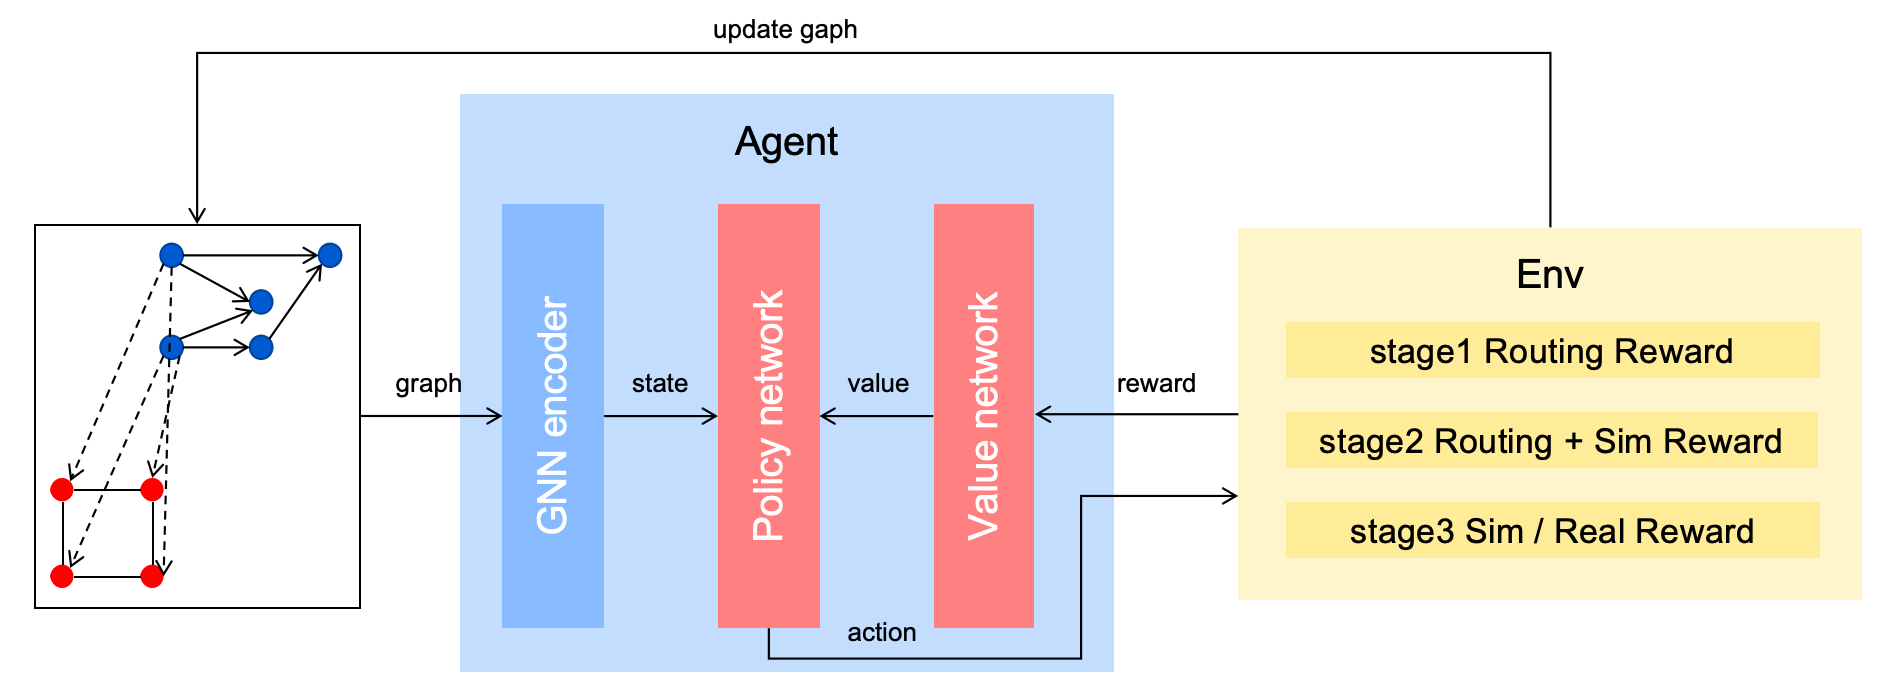
\includegraphics[width=0.95\textwidth]{body/routing/img/模型框架.jpg}
\caption{路由与映射联合优化系统总体框架}
\label{fig:routing-framework}
\end{figure}

如图~\ref{fig:routing-framework} 所示，系统整体构成「图编码—策略决策—噪声评估」的闭环流水线。左侧为输入编码层：逻辑电路被解析为 CircuitDAG（节点对应门操作，边对应数据依赖），硬件拓扑与噪声校准参数（T1/T2、逐边门错误率、串扰强度）被转化为 HardwareFeatures，二者按当前映射对齐为统一的图数据结构。中部为 SubGNN 编码器：多层多头 GAT 在电路依赖与物理耦合两种图结构上交替传播消息，为每个物理量子比特输出同时融合「线路角色」与「物理环境」信息的节点嵌入。右侧为 PPO 智能体：以边级 Actor-Critic 头为每条候选耦合边打分，在路由阶段执行物理 SWAP，在映射阶段执行虚拟 SWAP（见本章「映射：一种特殊的路由」小节）。底部为噪声模拟器：在 episode 终端以调度感知方式计算保真度，作为终端奖励回传给智能体，驱动 GNN 编码器与策略网络的端到端联合训练。

\subsubsection{CircuitDAG（电路有向无环图）}

\texttt{routing/graph/circuit\_dag.py} 将 QuantumCircuit 解析为 DAG 结构，每个节点对应一个门操作，边表示依赖关系。每个门记录其前驱门索引，支持拓扑排序和 front\_layer 提取（所有依赖条件已满足且未执行的双量子比特门）。特征编码输出 32 维节点特征和 16 维边特征。

\subsubsection{HardwareFeatures（硬件特征）}

\texttt{routing/graph/features.py} 从噪声配置构建硬件特征：包含物理距离矩阵、噪声参数（T1/T2、门错误率、串扰强度等），并提供 \texttt{RoutingGraphData} 数据结构作为 GNN 的 PyTorch Geometric Data 对象。

\subsubsection{SubGNN（图神经网络编码器）}

\texttt{routing/gnn/encoder.py} 实现基于 GATConv 的双向二分图编码器：
\begin{itemize}
  \item \textbf{输入}：32 维节点特征（逻辑/物理量子比特）、16 维边特征（门操作/物理连接）
  \item \textbf{架构}：3 层多头 GAT (hidden=64, heads=4) + LayerNorm + ReLU
  \item \textbf{输出}：\texttt{node\_embeddings()} 返回每个物理量子比特的 48 维嵌入
  \item \textbf{全局池化}：mean+max 池化得到 96 维全局嵌入
\end{itemize}

\begin{figure}[htbp]
\centering
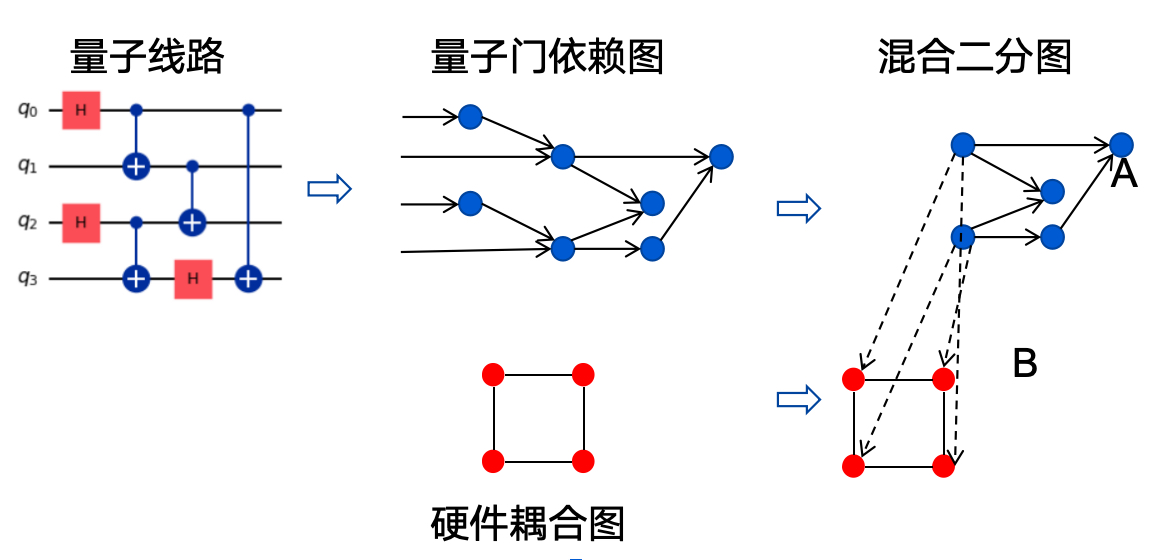
\includegraphics[width=0.9\textwidth]{body/routing/img/图编码.jpg}
\caption{电路结构与硬件拓扑的统一图编码}
\label{fig:graph-encoding}
\end{figure}

上述三个组件协同完成电路到图的编码，完整流程如图~\ref{fig:graph-encoding} 所示：电路侧每个门操作对应一个逻辑节点并携带门类型、作用比特等特征，门间数据依赖构成 DAG 的有向边；硬件侧每个物理量子比特对应一个物理节点并携带其 T1/T2、门错误率等噪声特征，物理耦合边上的边特征编码距离与串扰强度等信息（16 维）。逻辑节点与物理节点之间按当前映射 $\pi$ 建立对齐关系，使 GAT 的消息传播同时沿「门依赖」与「物理耦合」两个方向进行——一个物理比特的嵌入既反映经过它的门在电路中的位置与关键性，也反映其所在物理位置的噪声水平与邻域拓扑。该编码使得后续边级 $Q(s,a)$ 打分（见「RoutingEnv」小节）能够直接从节点嵌入中读取 SWAP 决策所需的全部结构性信息。

\subsubsection{RoutingEnv（强化学习环境）}

\texttt{routing/rl/env.py} 实现 Gymnasium 接口的环境。环境维护当前映射状态、已执行门集合、物理线路、调度时序和 X/Z 错误追踪，核心设计如下。

\textbf{观测空间}：每条耦合边独立构建局部特征向量，直接建模 $Q(s,a)$ 而非全局状态，解决了全局池化下的 state-action 歧义问题：

\[
\text{edge\_feat}_i = [h_p, h_q, h_p-h_q, \text{sabre\_feats}] \in \mathbb{R}^{149}
\]

其中 $h_p, h_q \in \mathbb{R}^{48}$ 为 GNN 节点嵌入，$\text{sabre\_feats} \in \mathbb{R}^5$ 为 SABRE 启发式特征，包含：
\begin{itemize}
  \item \texttt{front\_dist\_before}：执行 SWAP 前 front layer 门到目标边的归一化距离
  \item \texttt{front\_dist\_after}：执行 SWAP 后的距离
  \item \texttt{dist\_improvement}：距离改善量 $(d_{\text{before}} - d_{\text{after}}) / d_{\text{before}}$
  \item \texttt{num\_improved} / \texttt{num\_worsened}：距离改善/恶化的 front layer 门数量
\end{itemize}

完整观测为所有边的特征拼接，加上映射向量（每比特的物理位置编码）和进度标量（已执行门比例 + 映射阶段标志）。

\textbf{动作空间}：\texttt{Discrete(num\_edges + 1)}（映射阶段）或 \texttt{Discrete(num\_edges)}（纯路由阶段）。每个动作选择一条物理耦合边执行 SWAP，额外的 commit 动作触发映射阶段到路由阶段的切换。映射阶段的统一 MDP 设计见本章「映射：一种特殊的路由」小节。

\textbf{奖励函数}（Phase 1）：
\[
r_t = r_{\text{swap}} + \sum r_{\text{execute}} + \sum r_{\text{propagate}} + r_{\text{dist}}
\]
\begin{itemize}
  \item $r_{\text{swap}} = -0.3$：每次 SWAP 的固定代价
  \item $r_{\text{execute}}$：门执行奖励（CX=2.0，1Q=0.3--0.5）
  \item $r_{\text{propagate}}$：X/Z 错误传播惩罚
  \item $r_{\text{dist}} = -\eta \cdot (d_{\text{after}} - d_{\text{before}}) / \max(d_{\text{before}}, 1)$：距离缩短奖励（$\eta = 1.0$）
\end{itemize}

Phase 2 增加终端保真度奖励：$R_{\text{terminal}} = \lambda_{\text{fid}} \cdot F$，其中 $F$ 通过 Aer 密度矩阵仿真计算。

\textbf{死锁掩码}：检测最近 2 步内同一边的重复 SWAP 震荡，将该边屏蔽以防止无限循环。具体地，维护一个长度为 2 的滑动窗口记录最近执行的 SWAP 边索引，若当前候选边与窗口中的任一历史边相同，则将其从合法动作中排除。

\textbf{未映射比特掩码}：在映射阶段，尚未分配物理位置的逻辑比特对应的 SWAP 动作被屏蔽，确保映射按序进行。

\textbf{克隆方法}：\texttt{clone()} 返回环境的深拷贝，包括 DAG、映射、物理线路、调度时序、错误追踪等全部状态的独立副本，用于 beam search 推理时的状态模拟。克隆操作通过深拷贝和数组拷贝实现，确保副本间无共享可变状态。

\subsubsection{PPOAgent（策略智能体）}

\texttt{routing/rl/agent.py} 实现基于 PPO 的智能体：

\textbf{EdgeActorCritic 网络}：
\[
\text{score}_i = \text{MLP}_{\text{actor}}(\text{edge\_feat}_i) \in \mathbb{R}
\]
\[
\pi(a|s) = \text{softmax}([\text{score}_0, \ldots, \text{score}_{K-1}])
\]
Critic 使用注意力池化聚合边特征，降低输入维度至 155，提高训练稳定性。

\textbf{超参数}：$\text{lr}=3\times10^{-4}$, $\gamma=0.99$, $\lambda=0.95$, $\text{clip}=0.2$, $\text{entropy}=0.01$

\textbf{联合训练}：GNN 编码器参数纳入 PPO 优化器，实现 RL 驱动的端到端特征学习。

\subsection{噪声模拟器设计}
\label{sec:noise-simulator}

噪声模拟器是连接路由决策与物理硬件的桥梁：训练期为策略提供终端保真度信号（Phase 2 噪声感知奖励），评估期提供可信的保真度度量。系统以统一的噪声模型参数化为基础，实现了三级保真度求解器谱系——Aer 密度矩阵精确仿真、蒙特卡洛轨迹采样（支持调度感知演化）与解析保真度代理——按线路规模与精度需求选用。

\subsubsection{噪声模型}

NISQ 设备的门操作存在以下四类基本噪声：

\paragraph{退极化（Depolarizing）。} 每次门操作后，量子态有概率 $p$ 被随机施加一个 Pauli 矩阵。单比特门的恒等概率为 $1-3p/4$，X/Y/Z 各 $p/4$；双比特门的恒等概率为 $1-15p/16$，15 个非单位 Pauli 组合各 $p/16$。这建模了门操作的随机性错误。

\paragraph{热弛豫（Thermal Relaxation）。} 量子比特的 $|1\rangle$ 态会自发衰减到 $|0\rangle$ 态（T1 弛豫），概率为 $p_{\text{reset}} = 1 - e^{-t/T_1}$；叠加态的相对相位会随机漂移（T2 退相干），概率为 $p_z = 1 - e^{t/T_1 - 2t/T_2}$。这是时间依赖的噪声——比特空闲越久，衰减越严重。

\paragraph{ZZ 串扰（Crosstalk）。} 当两个物理比特在耦合图上相邻时，存在残余 ZZ 耦合 $H_{ZZ} = \theta \cdot Z \otimes Z$。当两对不相交的双比特门同时执行且其交叉比特相邻时，产生额外的相干错误。

\paragraph{读出错误。} 测量时比特状态翻转的概率，建模为对称错误矩阵。

\paragraph{噪声配置参数化。} 噪声配置通过 \texttt{NoiseConfig} 数据类参数化：

\begin{itemize}
  \item \texttt{t1\_times} / \texttt{t2\_times}：每个物理比特的 T1/T2 弛豫时间（$\mu$s）
  \item \texttt{single\_q\_gate\_error}：单比特门错误率（标量或逐比特列表）
  \item \texttt{two\_q\_gate\_error}：双比特门错误率（标量或逐边字典）
  \item \texttt{crosstalk\_strength}：ZZ 串扰强度（逐边字典，缺省为 $0.1 \times$ 双比特门错误率）
  \item \texttt{single\_gate\_time} / \texttt{two\_gate\_time}：门执行时间（$\mu$s）
\end{itemize}

逐比特/逐边的异质噪声参数同时进入 GNN 硬件特征与保真度计算。训练过程中，每个 episode 的噪声参数在标称值附近随机扰动（$\pm 20\%$），以增强策略对噪声变化的鲁棒性（见本章「噪声感知训练」小节）。

\subsubsection{Aer 密度矩阵仿真}

\texttt{NoiseSimulator} 基于 Qiskit Aer 构建完整的噪声模型（热弛豫、退极化、ZZ 串扰、读出错误），以密度矩阵求解器仿真线路。密度矩阵自然支持混合态与错误传播，是保真度评估的精确参考，但内存开销为 $O(4^n)$，仅适用于小规模线路（如 5 比特验证）的终端保真度计算。

\subsubsection{轨迹采样保真度}

精确的保真度评估通过蒙特卡洛轨迹采样实现（\texttt{TrajectorySimulator}）。对路由后的物理线路，执行 $T$ 条独立噪声轨迹，每条轨迹维护单个纯态状态向量（内存 $O(2^n)$），对每个噪声通道逐门做 Kraus 采样：

\begin{equation}
F = \frac{1}{T} \sum_{t=1}^{T} \left| \langle \psi_{\text{ideal}} | \psi_t \rangle \right|^2
\end{equation}

其中 $|\psi_t\rangle$ 为第 $t$ 条噪声轨迹的末态，$|\psi_{\text{ideal}}\rangle$ 为无噪声理想态。

轨迹采样的内存需求为 $O(2^n)$（纯态向量），相比密度矩阵的 $O(4^n)$ 大幅降低。20 量子比特时，密度矩阵需 16TB 内存，而轨迹采样仅需约 1KB。在相同噪声语义下，轨迹采样与 Aer 密度矩阵求解的保真度统计一致（误差 $<0.02$）。

\subsubsection{调度感知演化}

相同的量子线路，不同的门执行顺序和并行方式会产生不同的保真度。原因有三：

\paragraph{空闲退相干。} 比特在两次门操作之间的空闲期间持续经历 T1/T2 衰减。更好的调度将门排列得更紧凑，减少空闲时间，从而降低退相干累积。例如，串行调度中比特可能空闲数十微秒，而并行调度中空闲时间可降至门时长量级。

\paragraph{动态串扰。} 当两对不相交的双比特门在相邻耦合边上同时执行时，其交叉比特承受额外 ZZ 串扰。调度的并行度越高，串扰风险越大。这是并行度与保真度的 trade-off。

\paragraph{门时长差异。} 不同门的时长不同（CX 0.3$\mu$s，SWAP 0.9$\mu$s，rz 0$\mu$s）。长门执行期间，其他比特在空闲中累积退相干。

为此，调度感知轨迹模拟器以每门精确的 start/end 事件驱动噪声演化：事件序列直接取自环境的调度日志，与本章「门调度算法」小节的事件级 ASAP 调度器同源，保证训练奖励与评估口径一致。演化过程如下：

\begin{enumerate}
  \item 每比特维护独立时钟，门执行前对该比特的空闲区间施加热弛豫（Markov 精确复合，零时长事件前的等待期同样计账）
  \item 门执行期间按门类型与时长施加噪声：单比特门为退极化 + 热弛豫；CX/CZ 为双比特退极化 + 静态 ZZ 串扰 + 热弛豫；SWAP 物理上等价于 3 次 CX，施加相应强度的退极化、ZZ 串扰与热弛豫；零时长的参数化门只施加酉演化、不引入退相干
  \item 执行时间重叠的两对不相交门，其交叉比特在耦合图上相邻（1-hop）时，按实际重叠时长施加动态 ZZ 串扰（$\chi \cdot \Delta t$），并计入 1Q-2Q spectator 对
  \item 线路结束时，对仍空闲的比特补上末尾退相干
\end{enumerate}

这确保保真度评估忠实反映调度对噪声的影响：更好的调度产生更紧凑的门排列、更少的空闲退相干与更低的并行串扰。模拟器以 Qiskit DensityMatrix 与解析 Kraus 通道为精确参考完成对拍验证（端到端 $|\Delta F| < 0.02$）。

\subsubsection{物理比特截断优化}

路由后的物理线路可能仅使用了后端拓扑的部分量子比特。系统自动检测实际使用的量子比特子集，将线路和噪声参数裁剪到 $k$ 个比特（$k \leq n$），使状态向量模拟仅在 $2^k$ 空间上进行。在退极化 + 热弛豫 + ZZ 串扰模型下，未被作用的量子比特恒为 $|0\rangle$（$|0\rangle$ 是热弛豫的不动点），因此该裁剪对保真度精确等价，不引入近似。

\subsubsection{解析保真度代理}

为支持大规模线路（$\geq 16$ 量子比特）的训练，系统实现了 $O(G)$ 复杂度的解析保真度代理（$G$ 为门数），替代 $O(T \cdot G \cdot 2^n)$ 的轨迹采样：

\begin{equation}
\log F \approx \sum_{g \in C} \log(1 - \varepsilon_g)
\end{equation}

其中 $\varepsilon_g$ 为每条门的错误贡献，包括：
\begin{itemize}
  \item 退极化错误：$\varepsilon_{\text{depol}} = p$（门错误率）
  \item 热弛豫（可选）：$\varepsilon_{\text{th}} = \frac{t}{T_1} \cdot \frac{1}{2} + \frac{t}{T_2} \cdot \frac{1}{2}$
  \item ZZ 串扰（可选）：$\varepsilon_{\text{xtalk}} = \theta^2$（二阶近似）
\end{itemize}

该代理是一阶错误累积近似，忽略了门间错误的相干效应和调度差异，但保留了噪声参数的逐比特/逐边异质性。实测表明，对 19 量子比特线路，解析代理较轨迹采样（$T=16$）加速约 8000 倍（35.7s $\to$ 4.6ms），同时保真度相关性保持在合理范围。

\subsection{训练流水线}

系统采用两阶段课程训练策略：

\subsubsection{Phase 1：纯路由训练}

目标：学习高效路由策略，最小化 SWAP 数。
\begin{itemize}
  \item 时间步数：100,000
  \item 奖励模式：\texttt{routing}（无终端保真度信号）
  \item SABRE 距离特征 + 距离即时奖励 + 死锁掩码
  \item 数据集课程：Phase1 $\to$ Phase2 $\to$ Phase3（深度 2--13）
\end{itemize}

训练日志显示 entropy 从 1.38 降至 0.79（约 45K 步收敛），value loss 降至 0.1，SWAP 均值稳定在 4.6。

\subsubsection{Phase 2：噪声感知微调}

目标：在保持路由能力的同时优化保真度。
\begin{itemize}
  \item 加载 Phase 1 检查点
  \item 时间步数：100,000
  \item 奖励模式：\texttt{noise\_aware}（Aer 仿真保真度终端奖励）
  \item $\lambda_{\text{fid}}$ 从 0 线性退火至 5.0（前 50\% 步）
  \item 多拓扑混合：cross\_5q, ring\_5q, ibmq\_5\_line
\end{itemize}

全程 trunc=0\%，entropy 稳定在 0.79，value loss 0.06--0.29，fidelity 约 0.78。

\subsubsection{多规模课程学习}

为支持不同规模线路的泛化训练，系统实现了多规模课程学习策略。训练数据按量子比特数组织为独立的 split 文件：

\begin{itemize}
  \item \texttt{large\_n8\_phase1/2/3}：8 量子比特线路（150--300 条）
  \item \texttt{large\_n10\_phase1/2/3}：10 量子比特线路（150--300 条）
  \item \texttt{large\_n12\_phase1/2/3}：12 量子比特线路（150--300 条）
  \item \texttt{large\_n16\_phase1/2/3}：16 量子比特线路（300--500 条）
  \item \texttt{unified\_mixed}：8/10/12/16/20 量子比特混合线路（700 条）
\end{itemize}

课程通过 \texttt{--curriculum-keys} 参数控制，按训练进度自动切换数据集。例如，从 8 量子比特课程开始，待策略在当前规模收敛后，逐步过渡到 10、12、16 量子比特。每个规模的 Phase1/2/3 分别对应线路深度的浅/中/深三个层次。

\subsubsection{真机拓扑微调与调度感知训练}

面向真实硬件部署，系统在天衍 176 芯片的 20 比特连通子拓扑 tianyan176\_20q（以 Q23 为根 BFS 截取，20 比特 / 29 耦合边）上进行微调，噪声参数取自真机校准数据（逐比特 T1/T2 弛豫时间、逐边 CX 错误率）。工程上修复了真机噪声配置以字符串键序列化导致逐边错误率被静默丢弃的问题，修复后 28 个互异的逐边 CX 错误率才真正进入 GNN 特征与保真度计算。

训练开启事件级 ASAP 调度器（\texttt{--use-scheduler}），奖励在距离项之外叠加调度感知分量：总执行时长惩罚（$\eta_{\text{time}}$）、空闲退相干惩罚（$\eta_{\text{idle}}$）、并行度奖励（$\eta_{\text{parallel}}$）与 1-hop 动态串扰惩罚（$\eta_{\text{xtalk\_par}}$）。这使策略在压缩 SWAP 数的同时显式权衡 makespan、空闲退相干与串扰，而非单一优化路由长度。配合本章「映射：一种特殊的路由」小节介绍的 layout-mix 布局混合训练（恒等/随机/SABRE warm-start 按 $0.3/0.3/0.4$ 混合），得到最终主模型（l05）。

串扰建模上，动态串扰采用相干 ZZ 旋转 $e^{-i\theta Z\otimes Z}$（$\theta$ 取逐边串扰强度）而非概率性硬 $Z$ 翻转：后者对叠加态会造成正交归零式的失真惩罚，前者以 $\theta^2$ 量级平滑退化，与真实超导残余耦合的物理一致。同波并行的两对双比特门在其交叉比特于耦合图上相邻（1-hop）时施加该额外演化，与调度器强制同波比特互不相交的约束保持口径一致。

\subsubsection{噪声感知训练}

Phase 2 噪声感知微调的关键设计决策包括：

\paragraph{保真度信号来源。} 支持两种保真度计算方式：(1) 调度感知轨迹采样，对 $T=16$ 条独立噪声轨迹取平均，精确但计算量随量子比特数指数增长；(2) 解析保真度代理，一阶错误累积 $O(G)$ 复杂度，适用于 $\geq 16$ 量子比特的大规模线路训练（均见本章「噪声模拟器设计」小节）。

\paragraph{保真度奖励权重。} $\lambda_{\text{fid}}$ 控制保真度在总奖励中的比重。采用预热策略：前 50\% 训练步 $\lambda_{\text{fid}}$ 从 0 线性退火至最大值（默认 5.0），使策略先建立路由能力再引入保真度优化。$\lambda_{\text{fid}} = 0$ 时跳过保真度计算，减少训练开销。

\paragraph{保真度归一化。} 终端奖励中使用 per-size SABRE 基线保真度归一化：
\[
R_{\text{terminal}} = \lambda_{\text{fid}} \cdot \frac{F - F_{\text{sabre}}(n)}{1 - F_{\text{sabre}}(n)}
\]
其中 $F_{\text{sabre}}(n)$ 为 $n$ 量子比特线路的 SABRE 平均保真度。这使得不同规模线路的保真度奖励具有可比性。

\paragraph{噪声扰动。} 每个 episode 的噪声参数在标称值附近 $\pm 20\%$ 随机扰动，增强策略对噪声漂移的鲁棒性。训练过程使用 EMA（指数移动平均）权重定期在验证集上评估，保存最佳模型。

\subsection{Beam Search 推理}

为了弥补 PPO 前馈推理无法搜索的缺陷，实现了 1 步 Beam Search：
\begin{enumerate}
  \item 策略网络输出所有边的 logit 分数
  \item 选取得分最高的 K 个动作（默认 K=3）
  \item 对每个候选动作：克隆环境、执行虚拟 step、用 Critic 评估 $V(s')$
  \item 选取得分最高的动作执行真实 step
\end{enumerate}

\subsection{映射：一种特殊的路由}
\label{sec:mapping-as-routing}

\subsubsection{方法概述}

量子线路编译中的比特映射（初始布局选择）和路由（SWAP 插入）传统上被视为两个独立阶段：先用启发式算法（如 SABRE 的 \texttt{swap\_trials}）选择初始布局，再执行路由。这种分离忽略了布局质量与路由效率之间的耦合关系——一个好的初始布局可以显著减少路由阶段所需的 SWAP 数量，从而降低噪声累积。

本工作的视角是：映射本质上是一种特殊的路由。两者作用于同一物理耦合边集，动作形式同构——路由 SWAP 交换两个物理比特上的线路内容，映射 SWAP 仅重排逻辑比特到物理比特的映射向量，不写入物理线路、不递增 SWAP 计数、不引入噪声代价，可视为不落地的「虚拟路由」。由于映射与路由共享同一动作空间、同一观测编码与同一距离奖励结构，二者可以自然地统一到同一个强化学习 MDP 中联合优化：智能体在映射阶段通过虚拟 SWAP 学习初始布局，在路由阶段通过物理 SWAP 完成门调度，两个阶段共享同一个策略网络和 GNN 编码器。在此基础上，进一步引入布局混合训练策略（layout-mix）打通训练分布与推理分布：训练期按比例混合恒等、随机与 SABRE 预计算布局，使策略获得布局无关的路由能力，从而支持「SABRE 布局 + RL 路由」的 warm-start 混合推理管线。

\subsubsection{统一 MDP 设计}

\paragraph{统一动作空间。} 动作空间为 $\text{Discrete}(\text{num\_edges} + 1)$，其中：
\begin{itemize}
  \item 动作 $0 \sim \text{num\_edges} - 1$：对应物理拓扑上的耦合边 $(p, q)$，执行 SWAP 操作
  \item 动作 $\text{num\_edges}$：commit 动作，结束映射阶段并切换到路由阶段
\end{itemize}

观测向量为所有耦合边的局部特征拼接，末尾拼接映射向量（每比特的物理位置编码）、进度标量（已执行门比例）和 phase 标识符（映射阶段为 1.0，路由阶段为 0.0）。此外，映射阶段中尚未分配物理位置的逻辑比特对应的 SWAP 动作被屏蔽，确保映射按序进行。

\paragraph{虚拟 SWAP 机制。} 在映射阶段，智能体选择耦合边 $(p, q)$ 执行虚拟 SWAP（virtual SWAP）。虚拟 SWAP 仅重排逻辑比特到物理比特的映射关系：

\[
\text{mapping}[p] \leftrightarrow \text{mapping}[q]
\]

关键特性：
\begin{itemize}
  \item 不写入物理线路（\texttt{\_phys\_circuit} 不变）
  \item 不递增 SWAP 计数器（\texttt{\_swap\_counter} 不变）
  \item 不执行任何门操作
  \item 仅改变映射向量，为后续路由提供更好的初始布局
\end{itemize}

虚拟 SWAP 的距离缩短奖励与路由阶段相同：
\[
r_{\text{dist}} = -\eta \cdot \frac{d_{\text{after}} - d_{\text{before}}}{\max(d_{\text{before}}, 1)}
\]
其中 $d_{\text{before}}$ 和 $d_{\text{after}}$ 分别为虚拟 SWAP 前后 front layer 门到目标边的总距离。这使得智能体在映射阶段就能获得与路由阶段一致的距离信号，学习到什么样的布局能减少后续路由的 SWAP 需求。

\paragraph{阶段切换与自动执行。} 当智能体选择 commit 动作或映射预算耗尽时，映射阶段结束：
\begin{enumerate}
  \item 系统调用 \texttt{\_auto\_execute\_batch()}，自动执行所有前置条件已满足的门（即两个操作数物理相邻的门）
  \item 观测向量中的 phase 标识符从 1.0 变为 0.0
  \item 动作空间从 $\text{Discrete}(\text{num\_edges} + 1)$ 变为 $\text{Discrete}(\text{num\_edges})$（commit 动作不再合法）
  \item 进入路由阶段，智能体开始通过物理 SWAP 完成剩余门操作
\end{enumerate}

\paragraph{映射预算与布局质量惩罚。} 最大虚拟 SWAP 数为 $\text{mapping\_budget} = n - 1$（$n$ 为逻辑比特数），防止无限映射阶段。智能体也可以在预算内提前 commit，以平衡布局探索和路由效率。

在 commit 时刻，可选地施加布局质量惩罚：
\[
r_{\text{layout}} = -\lambda_{\text{layout}} \cdot \frac{1}{|F|} \sum_{g \in F} d(\pi(g.q_1), \pi(g.q_2))
\]
其中 $F$ 为当前 front layer，$\pi$ 为学到的映射，$d$ 为物理距离。该惩罚鼓励智能体在 commit 时已经将关键门的两个操作数放置在相邻或近距离的物理比特上。

\paragraph{布局混合训练策略（layout-mix）。} 仅有映射阶段机制还不够——训练分布同样决定策略能力。早期实验发现，若训练一律从恒等映射出发，策略会退化为「恒等布局专用」：评估时注入 SABRE 搜索到的优质初始布局做 warm-start，路由质量反而劣于恒等布局（SWAP 31.0 vs 27.5）。根因是策略从未见过非恒等初始布局，无法利用优质布局先验，路由能力被绑死在单一训练分布上。

为此，训练期引入布局混合采样（layout-mix）：每个 episode 按比例 $(\alpha_{\text{恒等}}, \alpha_{\text{随机}}, \alpha_{\text{SABRE}})$ 从三种布局源中抽取初始映射：
\begin{itemize}
  \item \textbf{恒等映射}：逻辑比特按序放置，保持原有路由能力（回归项）；
  \item \textbf{随机映射}：随机置换初始化，迫使策略学习与初始布局无关的路由能力；
  \item \textbf{SABRE 布局 warm-start}：从 SABRE 预计算的优质初始布局出发，训练策略在好布局上的精细化路由能力。
\end{itemize}

其中 SABRE 布局通过离线缓存预计算：对训练池全部电路以 \texttt{swap\_trials}=5 运行一次 SABRE 布局搜索并落盘缓存，训练期直接查表注入 \texttt{init\_mapping}，避免每个 episode 重复运行 SABRE 搜索的开销。消融实验（$\lambda_{\text{layout}} \in \{0, 0.5, 2.0\}$ 对照）表明收益主要来自训练分布多样性本身，commit 布局惩罚贡献很小（映射阶段平均仅消耗 0.1--0.8 次虚拟 SWAP）；$\lambda_{\text{layout}} = 0.5$ 略优，作为最终配置。

\paragraph{Warm-start 混合推理管线。} 布局混合训练解锁了「启发式布局 + 学习路由」的混合推理管线：评估时先用 SABRE 搜索初始布局，再由 PPO 策略从该布局出发完成路由。该管线将布局与路由解耦为各自最擅长的组件——SABRE 的 \texttt{swap\_trials} 多次采样擅长找好布局，RL 策略擅长在给定布局下做出噪声感知的 SWAP 决策。由于策略经 layout-mix 训练后具备了布局无关性，warm-start 输入不再造成分布偏移，反而稳定带来收益（详见实验章节）。

\subsubsection{与传统方法的对比}

\begin{table}[htbp]
\centering
\caption{映射方法对比}
\label{tab:mapping-comparison}
\small
\begin{tabular}{l|cc}
\hline
特性 & SABRE 映射 & 本工作（联合优化） \\
\hline
映射方法 & 启发式搜索（swap\_trials） & RL 策略学习 \\
布局选择 & 多次采样取最优 & 单次前馈推理 \\
布局-路由耦合 & 独立（布局固定后路由不变） & 联合（映射阶段可探索布局-路由交互） \\
布局先验利用 & 内生（自带布局搜索） & layout-mix 训练 + warm-start 混合管线 \\
噪声感知 & 仅通过保真度评估 & Phase 2 噪声感知微调 \\
泛化性 & 需要逐拓扑调参 & 多拓扑混合训练 \\
\hline
\end{tabular}
\end{table}

传统 SABRE 方法通过 \texttt{swap\_trials} 参数控制布局采样次数：对每个候选布局执行完整路由，选择 SWAP 数最少的布局。这种方法计算开销大（$O(\text{trials} \times \text{routing\_cost})$），且布局质量仅通过 SWAP 数间接评估。

本工作的联合优化方法将布局选择和路由统一到同一个 RL 训练流程中：映射阶段的虚拟 SWAP 奖励直接反映布局对后续路由的影响，策略网络通过端到端训练学习布局-路由的联合优化策略。训练完成后，映射和路由均通过单次前馈推理完成，计算效率显著提升。

需要强调的是，联合优化与启发式布局搜索并不互斥。经 layout-mix 训练后，本工作支持两种互补的部署形态：（1）\textbf{纯 RL 管线}——映射阶段 + 路由阶段均由策略单次前馈推理完成，推理开销最小；（2）\textbf{warm-start 混合管线}——SABRE 布局 + PPO 路由，在允许离线预计算布局的场景下进一步压低 SWAP 数并保持调度优势。消融实验（详见实验章节）表明，warm-start 管线在真机 20 比特拓扑上实现 SWAP 数与 SABRE 统计持平的同时，makespan 降至 SABRE 的 0.66 倍、串扰代价降至 0.45 倍、并行度提升至 1.6 倍，构成多目标严格占优。

\subsubsection{训练策略}

映射阶段的训练集成在本章的两阶段课程训练中：

\paragraph{Phase 1（纯路由 + 映射）。} 奖励函数包含虚拟 SWAP 的距离缩短奖励和 commit 时的布局质量惩罚。策略网络学习在映射阶段选择能减少后续路由 SWAP 需求的初始布局。最终主模型（l05）在真机 tianyan176\_20q 拓扑上以调度感知奖励微调，配置为：布局混合比例 $0.3/0.3/0.4$（恒等/随机/SABRE warm-start）、$\lambda_{\text{layout}} = 0.5$、SABRE 布局缓存 \texttt{trials}=5、事件级 ASAP 调度器开启、10 万时间步。

\paragraph{Phase 2（噪声感知微调）。} 在 Phase 1 检查点基础上，增加终端保真度奖励。策略网络进一步学习在噪声环境下选择能提高最终保真度的布局-路由策略。

训练采用多拓扑课程（基础拓扑预训练 $\to$ 真机子拓扑微调），增强策略对真实硬件噪声异质性的适应能力。映射预算为 $n - 1$，布局混合策略（\texttt{--layout-mix}）在训练中按比例随机使用恒等映射、随机映射和 SABRE 映射作为初始状态，迫使策略学习与初始布局无关的路由能力；该能力是 warm-start 混合推理管线得以生效的前提。

\subsection{测试情况}

当前共有 3 个测试文件，18 个测试用例全部通过：

\begin{itemize}
  \item \textbf{test\_circuit\_dag.py}（5 个测试）：DAG 解析、图特征张量形状、串扰特征、PyG Data 转换
  \item \textbf{test\_env.py}（12 个测试）：观测空间、动作执行、奖励计算、噪声感知模式、死锁掩码、错误追踪
  \item \textbf{test\_eval\_phase1.py}（1 个慢测试）：端到端模型评估，验证 PPO 在三个拓扑上 100\% 完成，SWAP 数低于 Greedy
\end{itemize}
